\documentclass[border=10pt]{standalone}

\usepackage[utf8]{inputenc}
\usepackage[english]{babel}
\usepackage{tikz}
\usetikzlibrary{positioning, arrows.meta, fit}

\tikzset{%
  every neuron/.style={
    circle,
    draw,
    minimum size=1cm
  }
}



\begin{document}
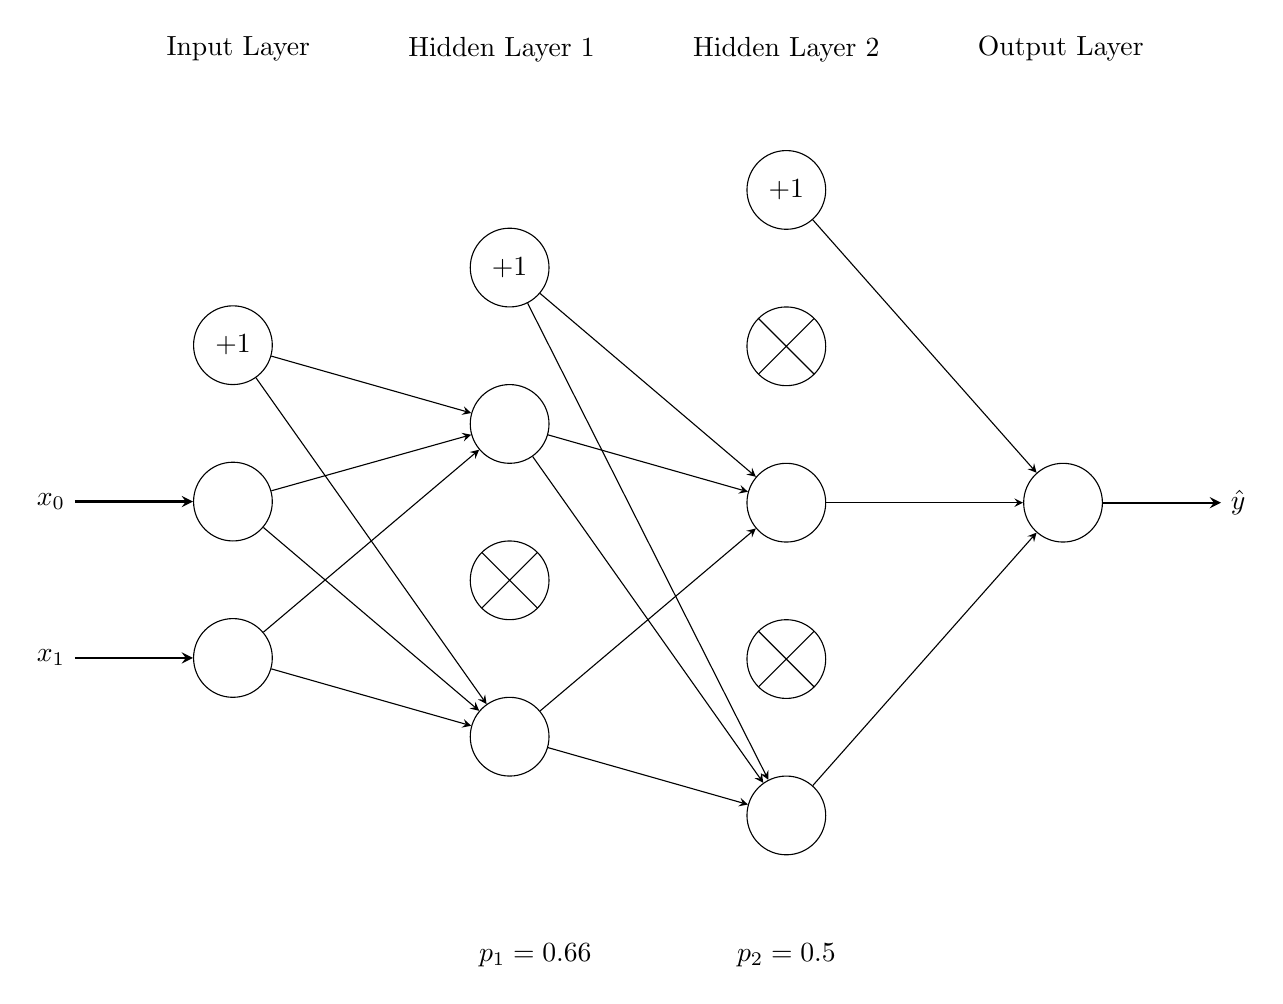
\begin{tikzpicture}[>=stealth,cross/.style={path picture={ 
  \draw[black]
  (path picture bounding box.south east) -- (path picture bounding box.north west) (path picture bounding box.south west) -- (path picture bounding box.north east); }}]
		%% input layer
		\node[every neuron] (a01) {};
		\node[every neuron, yshift=4cm, below=of a01] (a00) {};
		\node[every neuron, yshift=4cm, below=of a00] (b0) {$+1$};
		\node[xshift=-0.5cm, left=of a01] (x1) {$x_1$};
		\node[xshift=-0.5cm, left=of a00] (x0) {$x_0$};
		\draw[-stealth, thick] (x1) -- (a01);
		\draw[-stealth, thick] (x0) -- (a00);
		%% hidden layer 1
		\node[every neuron, yshift=-1cm, xshift=1.5cm, right=of a01] (a12) {};
		\node[every neuron, yshift=4cm, below=of a12, cross] (a11) {};
		\node[every neuron, yshift=4cm, below=of a11] (a10) {};
		\node[every neuron, yshift=4cm, below=of a10] (b1) {$+1$};
		%% hidden layer 2
		\node[every neuron, yshift=-1cm, xshift=1.5cm, right=of a12] (a23) {};
		\node[every neuron, yshift=4cm, below=of a23, cross] (a22) {};
		\node[every neuron, yshift=4cm, below=of a22] (a21) {};
		\node[every neuron, yshift=4cm, below=of a21, cross] (a20) {};
		\node[every neuron, yshift=4cm, below=of a20] (b2) {$+1$};
		%% output layer
		\node[every neuron, xshift=1.5cm, right=of a21] (a30) {};
		\node[xshift=0.5cm, right=of a30] (y) {$\hat{y}$};
		\draw[-stealth, thick] (a30) -- (y);
		%% description
		\node[above=of b2] (hl2) {Hidden Layer 2};
		\node[right=of hl2] (ol) {Output Layer};
		\node[left=of hl2] (hl1) {Hidden Layer 1};
		\node[left=of hl1] (il) {Input Layer};
		\node[below=of a23] (h2) {$p_2 = 0.5$};
		\node[left=of h2, xshift=-0.6cm] (h1) {$p_1 = 0.66$};
		%% input layer connections
		\path [->] (b0) edge node [auto] {} (a10);
		%\path [->] (b0) edge node [auto] {} (a11);
		\path [->] (b0) edge node [auto] {} (a12);
		% input0
		\path [->] (a00) edge node [auto] {} (a10);
		%\path [->] (a00) edge node [auto] {} (a11);
		\path [->] (a00) edge node [auto] {} (a12);
		% input1
		\path [->] (a01) edge node [auto] {} (a10);
		%\path [->] (a01) edge node [auto] {} (a11);
		\path [->] (a01) edge node [auto] {} (a12);
		%% hidden layer 1 connections
		%\path [->] (a10) edge node [auto] {} (a20);
		%\path [->] (a11) edge node [auto] {} (a20);
		%\path [->] (a12) edge node [auto] {} (a20);
		%\path [->] (b1) edge node [auto] {} (a20);
		\path [->] (a10) edge node [auto] {} (a21);
		%\path [->] (a11) edge node [auto] {} (a21);
		\path [->] (a12) edge node [auto] {} (a21);
		\path [->] (b1) edge node [auto] {} (a21);
		%\path [->] (a10) edge node [auto] {} (a22);				
		%\path [->] (a11) edge node [auto] {} (a22);
		%\path [->] (a12) edge node [auto] {} (a22);
		%\path [->] (b1) edge node [auto] {} (a22);
		\path [->] (a10) edge node [auto] {} (a23);
		%\path [->] (a11) edge node [auto] {} (a23);
		\path [->] (a12) edge node [auto] {} (a23);
		\path [->] (b1) edge node [auto] {} (a23);
		%% hiden layer 2 connection
		%\path [->] (a20) edge node [auto] {} (a30);
		\path [->] (a21) edge node [auto] {} (a30);
		%\path [->] (a22) edge node [auto] {} (a30);
		\path [->] (a23) edge node [auto] {} (a30);
		\path [->] (b2) edge node [auto] {} (a30);
	\end{tikzpicture}
\end{document}